\section{Oscillation analyzed via the principal value integral}\label{sec::oscillation}

Here we are trying to explain the oscillatory property of the integral given by
\begin{equation}
    I_o = \int_0^{\infty} \frac{J_0(k \D \rho) \exp{(-k a)}}{\exp{(2H(k_0 - k))} - 1} \text{d}k\;,
\end{equation}
where~$k_0$,~$a$ and~$\rho$ are all positive constants.
The integral can further be divided via Laurent expansion, given by
\begin{equation}
    I_o = \int_0^{\infty} \frac{J_0(k \D \rho) \exp{(-k a)}}{2H(k_0 - k)} \text{d}k + \int_0^{\infty} J_0(k \D \rho) \exp{(-k a)} E(k) \text{d}k\;,
\end{equation}
where~$1/2H(k_0 - k)$ is the leading order term of the Laurent series of~$\frac{1}{e^{2H(k_0 - k)} - 1}$, and~$E(k)$ is the Padé approximant of the rest part, which is a non-divergent smooth function.
Due to the fast decay property of~$\exp{(-k a)}$, the second part leads to a non-oscillatory small contribution to the result, and the oscillation is contributed by the leading order term.

To calculate the integral, we treat it as a function of~$a$, given by
\begin{equation}
    I_{o1}(a) = \int_0^{\infty} \frac{J_0(k \D \rho) \exp{(-k a)}}{2H(k_0 - k)} \text{d}k\;,
\end{equation}
so that we have
\begin{equation}
    \begin{split}
    I_{o1}^{\prime}(a) & = - k I_{o1}(a) = \frac{1}{2H} \int_0^{\infty} J_0(k \D \rho) \exp{(-k a)} \text{d}k - k_0 I_{o1}(a) \\
    & = \frac{1}{2H \sqrt{\D \rho^2 + a^2}} - k_0 I_{o1}(a) \;,
    \end{split}
\end{equation}
which forms a differential equation given by
\begin{equation}
    I_{o1}^{\prime}(a) + k_0 I_{o1}(a) = \frac{1}{2H \sqrt{\D \rho^2 + a^2}}\;.
\end{equation}
Using the general solution of ODE, we have
\begin{equation}
    I_{o1}(a) = \exp{(-k_0 a)} \left[C_1 + \int \frac{\exp{(k_0 a)}}{2H \sqrt{\D \rho^2 + a^2}} \text{d}a \right] = \exp{(-k_0 a)} \left[C_1 + C_2(\rho, k_0, a) \right] \;.
\end{equation}
Notice that
\begin{equation}
    I_{o1}(0) = C_1 + C_2(\D \rho, k_0, 0)\;,
\end{equation}
so that
\begin{equation}
    I_{o1}(a) = \exp{(-k_0 a)} \left[ I_1(0) - C_2(\D \rho, k_0, 0) + C_2(\D \rho, k_0, a) \right]\;.
\end{equation}
Although here we do not know the exact result of integral~$C_2$, its contribution to~$I_{o1}$ is clearly non-oscillatory.
Then we can focus on the first term, which contribute the oscillation, given by 
\begin{equation}
    I_{o2} = \frac{\exp{(-k_0 a)}}{2H} \int_0^{\infty} \frac{J_0(k \D \rho)}{(k_0 - k)} \text{d}k = \frac{\exp{(-k_0 a)}}{2H} \int_0^{\infty} \frac{J_0(k^\prime)}{k_0 \D \rho - k^\prime} \text{d}k^\prime\;,
\end{equation}
so that 
\begin{equation}
    I_o = \frac{\exp{(-k_0 a)}}{2H} \int_0^{\infty} \frac{J_0(k^\prime)}{k_0 \D \rho - k^\prime} \text{d}k^\prime + f(k_0, \D \rho, a)\;.
\end{equation}
where~$f(k_0, \D \rho, a)$ is a non-oscillatory function defined by
\begin{equation}
    \begin{split}
        f(k_0, \D \rho, a) = & \exp{(-k_0 a)} \left[ - C_2(\D \rho, k_0, 0) + C_2(\D \rho, k_0, a) \right] \\
        & + \int_0^{\infty} J_0(k \D \rho) \exp{(-k a)} E(k) \text{d}k
    \end{split}
\end{equation}
Here we define
\begin{equation}
    I_{m} = \int_0^{\infty} \frac{J_0(k^\prime)}{k_0 \D \rho - k^\prime} \text{d}k^\prime\;,
\end{equation}
which is only related to~$k_0 \D \rho$, and the numerical result shows that distance between ~$I_{m}$ converge rapidly to~$\pi$, as shown in Fig.~\ref{fig:I_3}.

\begin{figure}[htbp]
\centering
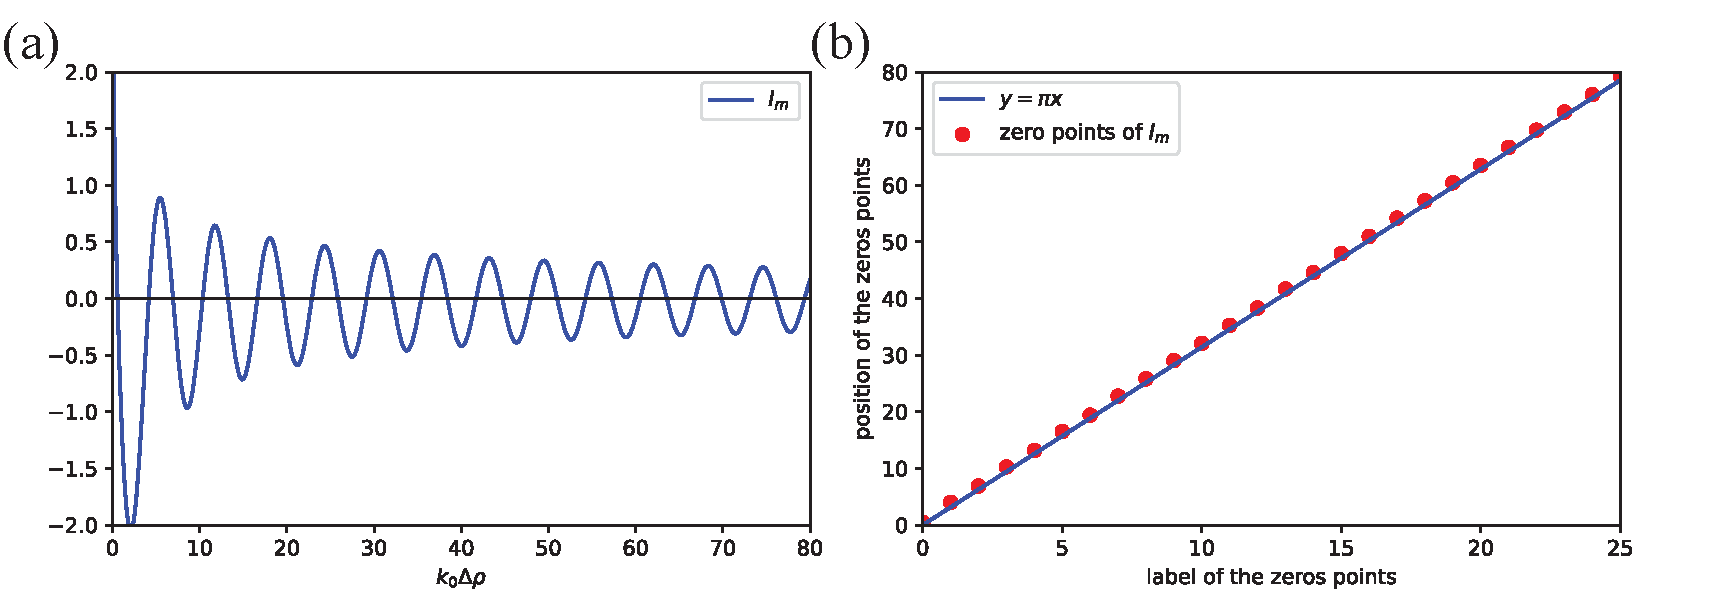
\includegraphics[width=  \linewidth]{figs/I_3.pdf}
\caption{
    Numerical results of~$I_{m}$ is shown in (a), and the position of the zero points are shown in (b).
}
\label{fig:I_3}
\end{figure}


\section{Simulation details}

In the main text, we have shown that the charge oscillation can lead to lattice-like structure formation in dielectric confined quasi-2D systems, and mainly focused on the tunable lattice parameter.
Here we will discuss more about our results.

\begin{figure}[ht]
    \centering
    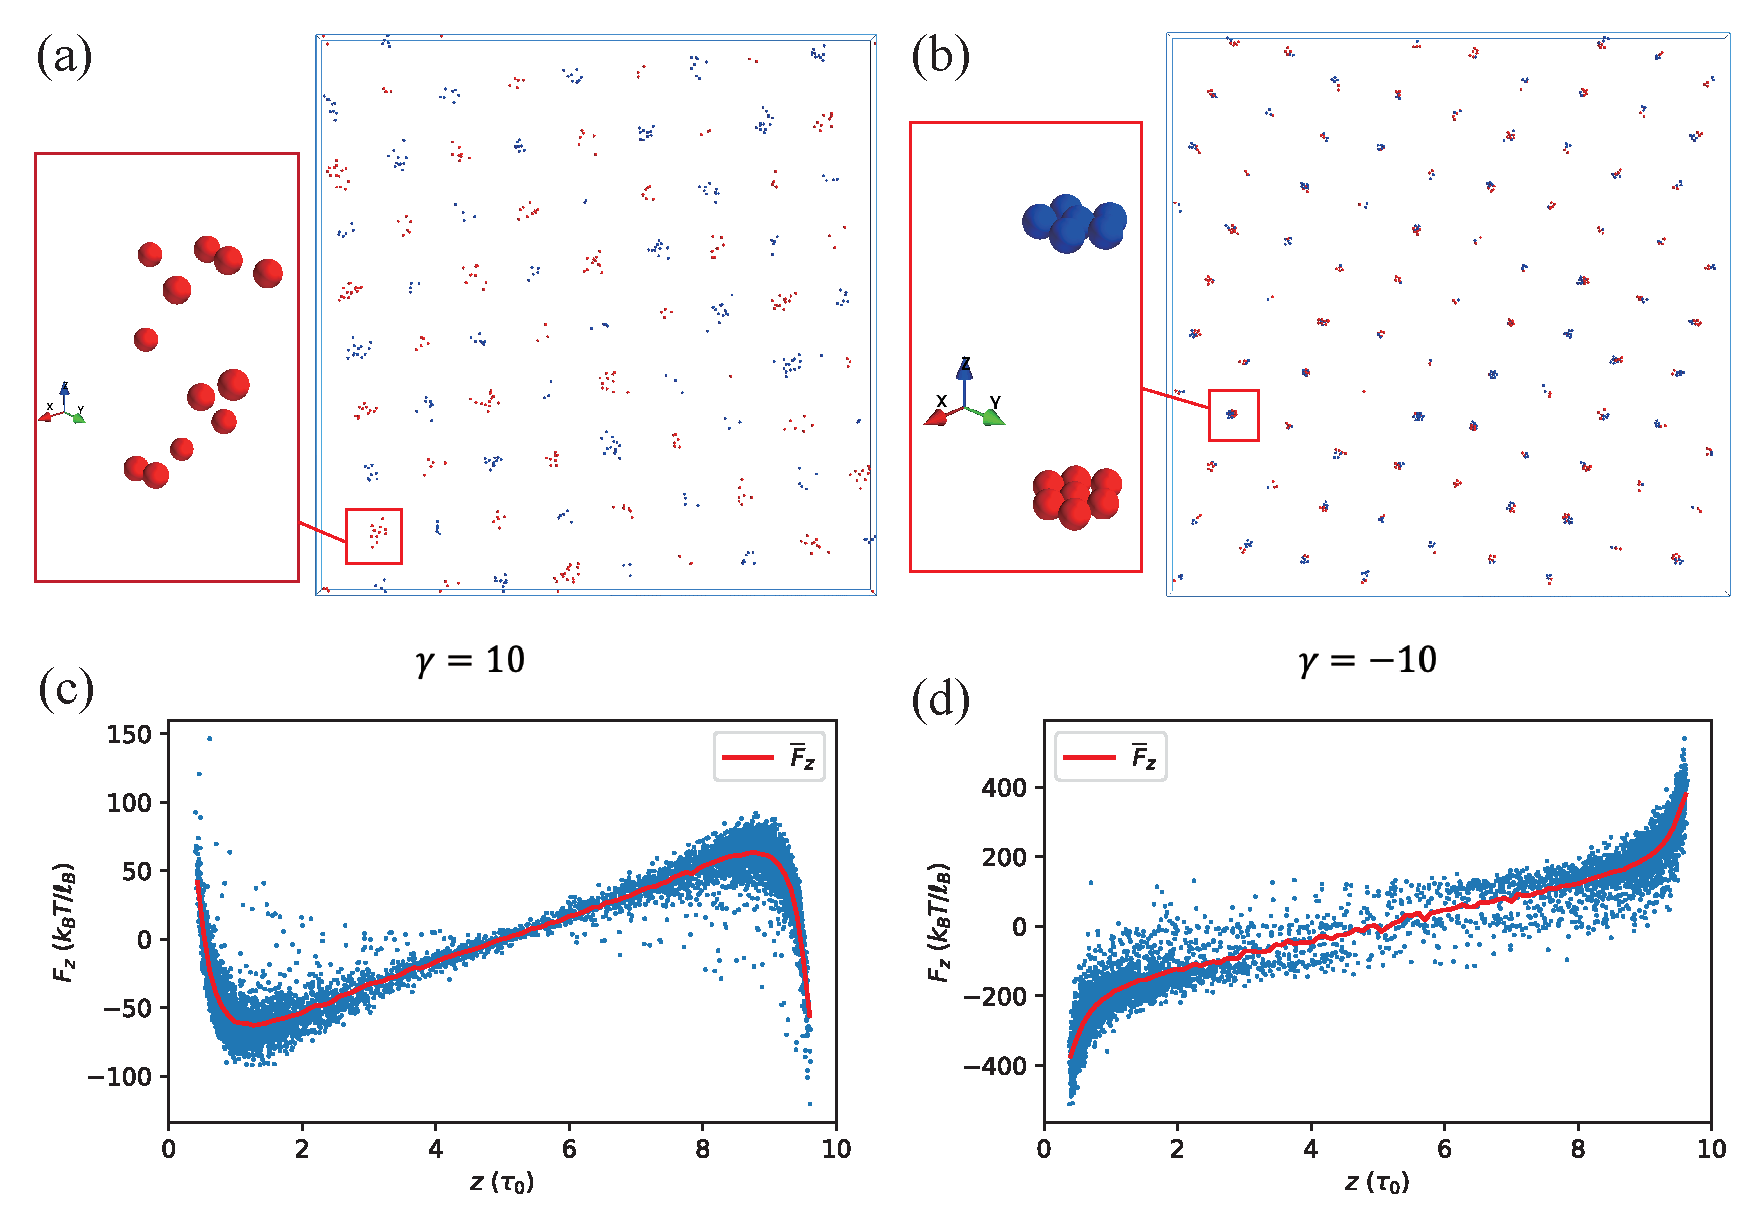
\includegraphics[width = \linewidth]{figs/MD_ball.pdf}
    \caption{The lattice-like structure and the cluster for~$\gamma = \pm 10$ cases are shown in (a) and (b), respectively. Force in~$z$ direction on particles at different position are shown in (b).}
    \label{fig:balls}
\end{figure}

The MD results for the systems which contain~$600$ particles is shown in Fig.~\ref{fig:balls} (a) and (b), and the related videos are given as video1 and video2.
For both simulations, it costs $2 \times 10^6$ time steps in total, and each step takes~$\Delta t = 0.005 t_0$, where~$t_0 = \tau_0 \sqrt{\frac{m_0}{k_B T}}$ is the reduced time scale.
The first $1.5\times 10^6$ steps are performed using the simulated annealing technique to avoid trapping in a metastable state. We start with $T_r=10$ and slowly cooling down the system until it reaches equilibrium at $T_r=1$, after which we continue the simulation for $5 \times 10^5$ time steps for sampling.

The ions distribute near the substrates and pair with other ions on the opposite side.
For~$\gamma = 10$ and~$-10$ cases, the pairs are symmetric and anti-symmetric, respectively, as shown in the sub-figure.
The difference come from the sign of the reflection rate, which determines whether the polarized charges at opposite positions are of the same sign or of different sign, thus determines the symmetry of the ions on the opposite sites.

Shapes of the clusters are also different.
For both cases, we attribute the cluster formation to the strong polarization charge with different sign on the substrate as shown in Fig.~1~(a) of the main text, which form a deep potential well and trapped these ions inside.
In the transverse direction, when~$\gamma = 10$, the ions forms ion liquid and separate from each other, and when~$\gamma = -10$, the ions are closely packed, because of the force in transverse direction between ions with the same sign are repulsive or attractive at short range, respectively.
In the vertical direction, we calculated forces in~$z$ to explain the distributions obtained, as shown in Fig.~\ref{fig:balls} (c) and (d).
When~$\gamma = 10$, we found that the surface with opposite sign reverse the force in the middle region and pull the ions to the substrates, so that the ions are distributed near the substrates but not closely touching.
When~$\gamma = -10$, the force is purely attractive and the ions are all closely attached to the substrates.